\begin{problem}{/images/problems/pic.jpg}{Pipe Drilling}
	The red curve here is defined by $y = 2x^2$ and the circle is surrounded by the curve and the line $y=1$. What are the coordinates of the center of the circle and the radius of the circle?

\begin{center}
	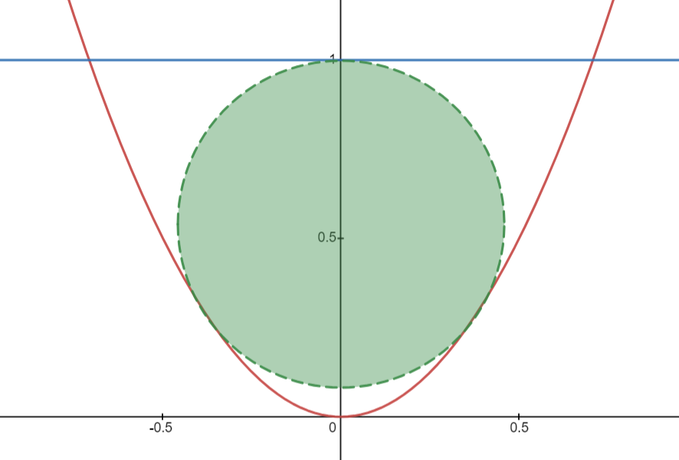
\includegraphics{/images/problems/41_pipe.png}
\end{center}

Link to the problem on Twitter: \url{https://twitter.com/Riazi_Cafe/status/1705827665717137521}
\end{problem}
\begin{solution}
The center of the circle is approximately equal to $(0,0.542)$ and radius of the circle is approximately equal to 0.4571.\\[0.2cm]

According to the definition, the curve $y=2x^2$ is the geometric location of the points that are of the same distance from the focus with coordinates $F: (x=0, y=1/8)$ and the directrix with the relation $y=-1/8$.
Therefore, in the diagram below, $\bar{FP}=\bar{AP}$ and their adjacent angles in the formed triangle are equal.

Also, by the symmetry of parabola, the segments $BP$ and $FP$ make an equal angle with the segment perpendicular to the parabola at the point $P$, and according to the property of the circle, the segment perpendicular to the point $P$ is the radius of the circle.

Thus the angles marked in the figure are equal, and $CFAP$ is a parallelogram, and therefore $\bar{CF}=\bar{AP}$, from which we can conclude $C_y=P_y+1/4$.

$$\begin{aligned}
CF = AP \implies& \\
C_y - F_y = P_y - A_y \implies& \\
C_y - \frac{1}{8} = P_y + \frac{1}{8} \implies& C_y=P_y+\frac{1}{4}
\end{aligned}$$

\begin{center}
	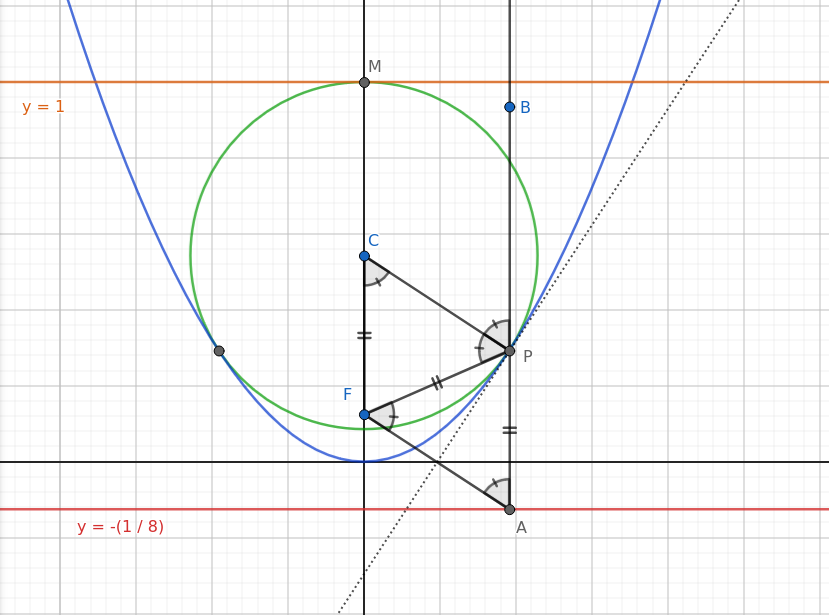
\includegraphics{/images/problems/41_diagram0.png}
\end{center}

On the other hand, the radius of the circle is equal to $1-C_y$. Therefore $\bar{CP}=1-C_y$. If we put this next to $C_y=P_y+1/4$, we can determine $C_y$ and $R$.

$$\begin{aligned}
CM = CP \implies& (1 - C_y)^2 = (C_y - P_y)^2 + (0 - P_x)^2 \\
\implies& (1 - C_y)^2 = \frac{1}{4}^2 + \frac{P_y}{2} \\
\implies& 1 - 2C_y + C_y^2  = \frac{1}{4}^2 + \frac{C_y-1/4}{2} \\
\implies& C_y^2 - \frac{5}{2}C_y + \frac{17}{16} = 0 \\
\implies& C_y = \frac{5}{4} - \frac{1}{\sqrt{2}}, R = \frac{1}{\sqrt{2}} - \frac{1}{4}
\end{aligned}$$


\end{solution}